\chapter{Evaluation \& Results}

In this chapter we explained how the evaluation of the developed tasks and systems was done.

\section{Sentiment analysis evaluation}

As mentioned previously, the semtniment analysis task was trained using a dataset from Stanford. To perform this task we used the same test and train splits used in \cite{socher2013recursive} which is the same from \cite{DBLP:journals/corr/Kim14f}. During training, both the loss and the accuracy of this classification task were recorded but only the loss is used in back-propagation.

The loss function was choosen among the ones available in the Keras framework to be the categorical cross-entropy \cite{golik2013cross} and the optimizer was Adadelta \cite{zeiler2012adadelta}. The batch size was set to 50 to stay as close as possible to the experiment conditions from \cite{DBLP:journals/corr/Kim14f}.

\begin{figure}[h]
    \centering
    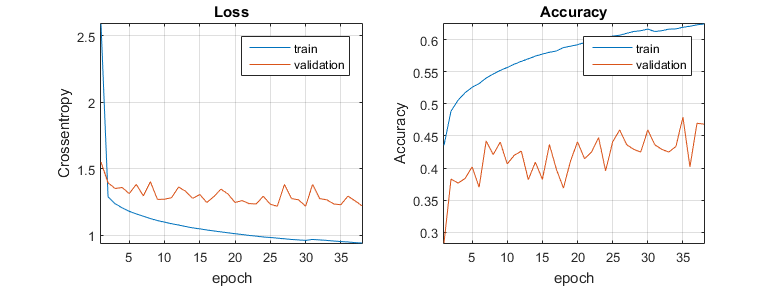
\includegraphics[width=16cm]{figures/sa}
    \caption{Training and validation curves of the sentiment analysis task.}
\end{figure}

\section{Speech synthesis evaluation}

This section contains both the objective and subjective evaluation results and how they were performed. A total of three experiments wert evaluated. These experiments are:

\begin{enumerate}
    \item Baseline system (only linguistic features from section \ref{sec:ling-feat})
    \item Embeddings without doing the domain adaptation.
    \item Embeddings but with the domain adaptation.
\end{enumerate}

\subsection{Objective evaluation}

%Training curves of the different stages of this project (accuracy \& loss curves) as well as objective metrics from  the work proposal document.
To perform the objective evaluation the Socrates framework keeps track of the loss evolution during the training. At the end of each batch, it saves the batch loss and at the end of each epoch, the validation data is used to obtain the validation loss of the models.

The metric that are computed by Socrates are the root mean square error (RMSE) for the duration predictions, mel cepstral distortion \cite{mashimo2001evaluation} (MCE) for the MFCC predictions, RMSE for the $F_0$ predictions and accuracy (\%) for the UV flag. 

\begin{table}[h]
    \centering
    \begin{tabular}{|l|c|c|c|c|}
        \hline
                     & Duration &  MFCC & $F_0$ & UV \\
        \hline
        Random weights  & 152.75   & 22.35 & 58.50 & 34.31 \\
        Baseline     & 49.17    & 7.18  & 37.67 & 95.32 \\
        Expressive embeddings     & 51.76    & 7.35  & 41.46 & 94.72 \\
        Adapted embeddings     & 49.37    & 8.24  & 42.04 & 66.28 \\
        \hline
    \end{tabular}
    \caption{Objective metrics.}
\end{table}

Both the duration and acoustic models were trained minimizing the mean square error (MSE) using the Adam \cite{kingma2014adam} optimizer.

\begin{figure}[h]
    \centering
    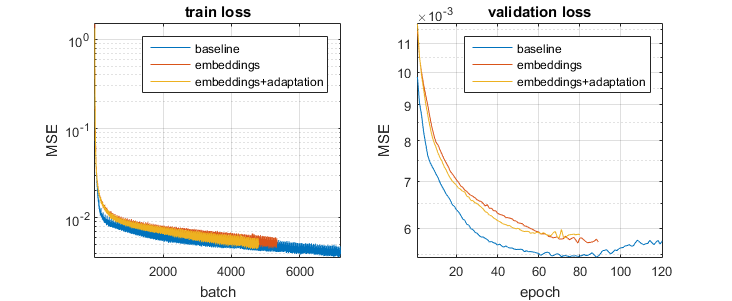
\includegraphics[width=14cm]{figures/duration}
    \caption{Duration model's training curves}
\end{figure}

\begin{figure}[h]
    \centering
    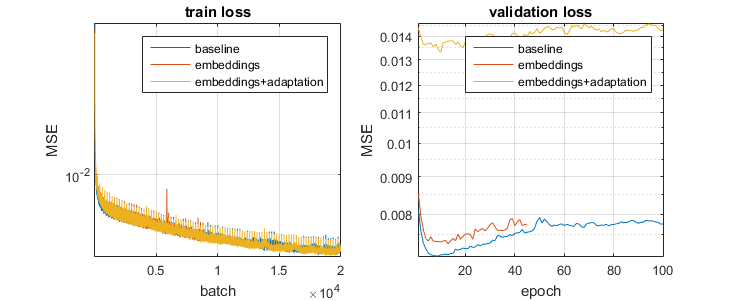
\includegraphics[width=14cm]{figures/aco}
    \caption{Acoustic model's training curves}
\end{figure}

\subsection{Subjective evaluation}

%Results from the subjective evaluation. Box plots comparing experiments.
To perform the subjective evaluation, six sentences were chosen from the test split from the Blizzard corpus. To choose the sentences, all the transcripts from the corpus were processed with the sentiment analysis classifier from Section \ref{sec:sa} and a score was computed for each of them:

\begin{equation}
    s = 2 \cdot p_{nn} + \cdot p_{n} - \cdot p_{p} - 2 \cdot p_{pp}
\end{equation}

Where $p_{nn}$ is the probability of the sentence being \textit{very negative}, $p_n$ is the probability of being \textit{negative}, $p_p$ is the probability of the sentence being \textit{positive} and $p_{pp}$ is the probability of being \textit{very positive}. The probability of a sentence being \textit{neutral} is not used in the score.

The scored sentences were sorted in a list and two were picked from the top (as negative sentences), two from the bottom (positive sentences) and two from the middle (neutral sentences).

A web based application (Figure \ref{fig:webapp}) was developed with the selected audio files obtained from the systems from Section \ref{sec:systems} and volunteers were asked to rate how appropriate the voices were in a scale from one to five, one being \textit{very unappropriate} and five being \textit{very appropriate}. The results were saved in an SQL database in the server side of the application.

The test was performed by a total of eight volunteers who gave a rating to all the samples, therefore we end up having a total of forty-eight subjective evaluations for each of the three experiments. Figure \ref{fig:boxplot0} contains a box plot of the collected data:

\begin{figure}[h]
    \centering
    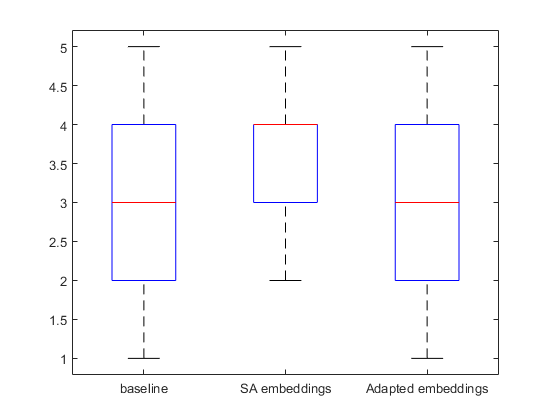
\includegraphics[width=10cm]{figures/box0}
    \caption{Subjective evaluation results.}
    \label{fig:boxplot0}
\end{figure}

\begin{figure}
    \centering
    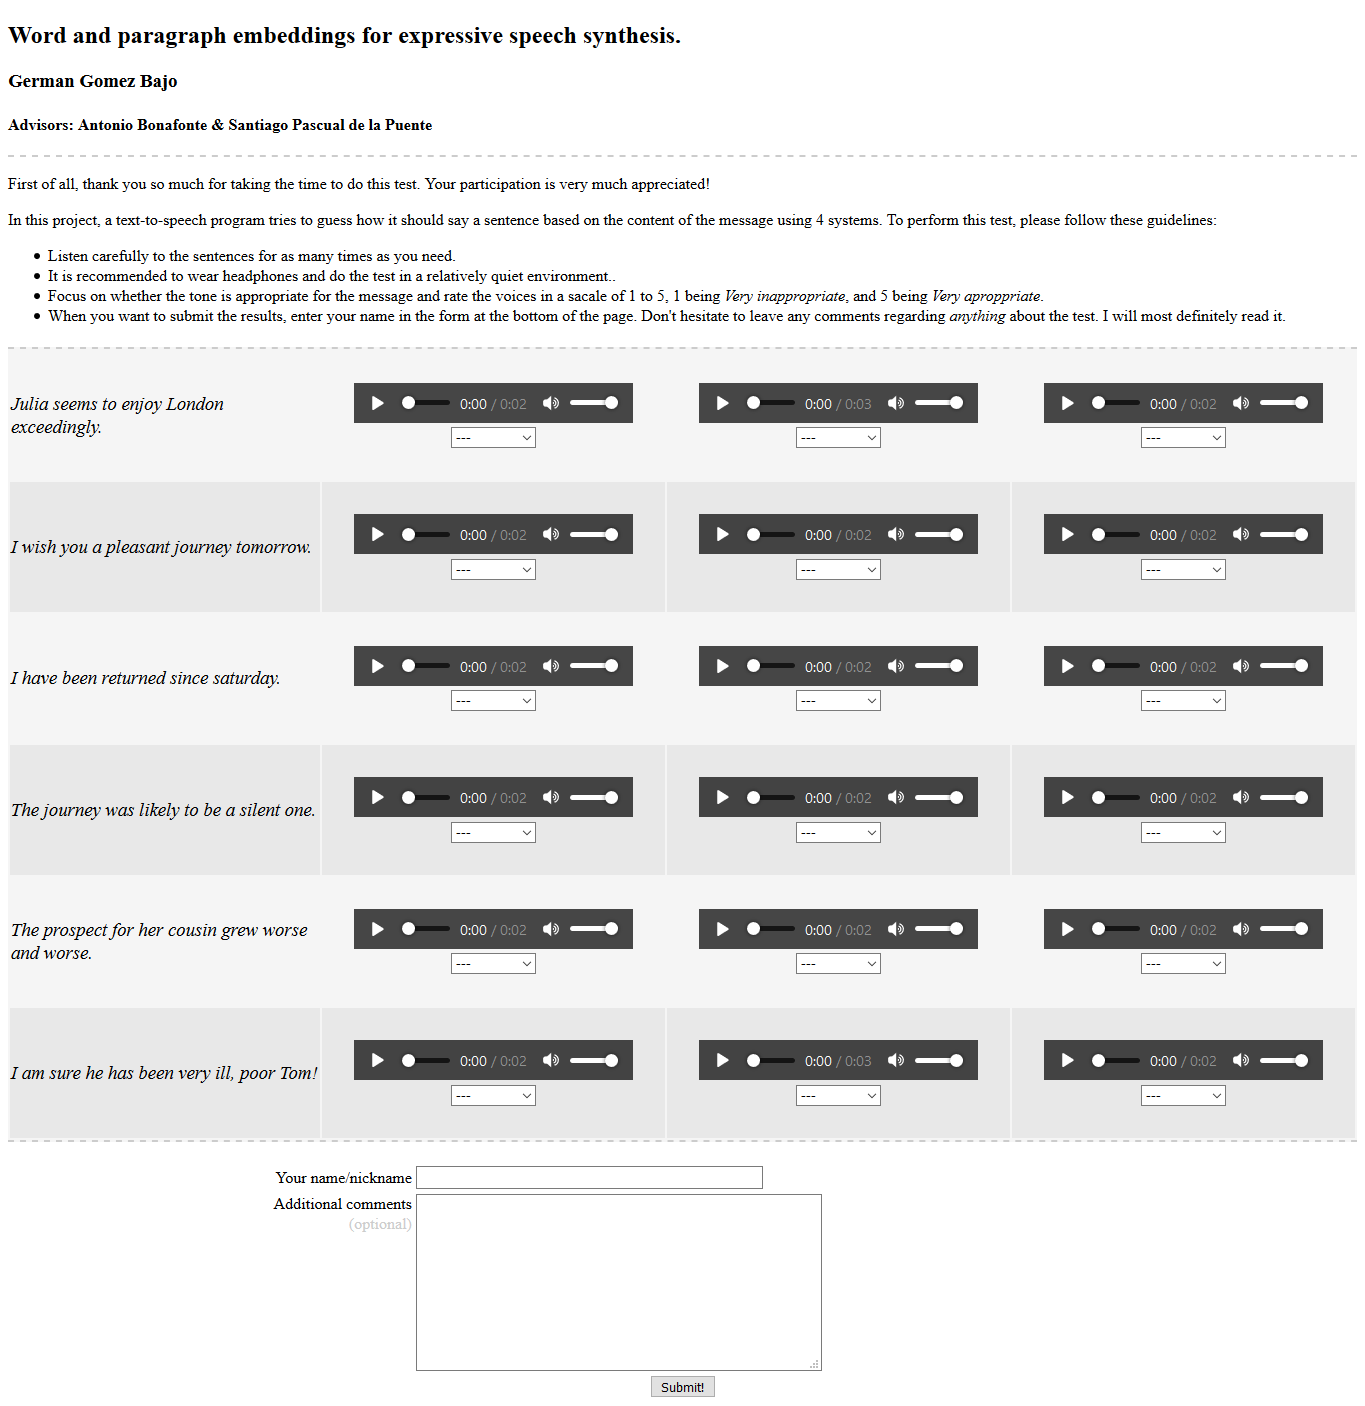
\includegraphics[width=16cm]{figures/webapp}
    \caption{Screenshot of the subjective evaluation's web application.}
    \label{fig:webapp}
\end{figure}
